%!TEX TS-program = xelatex
\documentclass[vi]{hnue-thesis} % use [vi] for vietnamese

\usepackage[utf8]{inputenc}
\usepackage{ upgreek }
\usepackage{blindtext}
\usepackage{ tipa }
\usepackage{indentfirst}
\usepackage{dsfont}
\usepackage{tikz}
\usepackage{tikz-cd}

\title{ĐỊNH LÝ CẮT BỎ TRONG LÝ THUYẾT ĐỒNG ĐIỀU KỲ DỊ}
\author{Nguyễn Trường Nhi}
\authoremail{nguyentruongnhi2801@gmail.com}
\major{Hình học}
\field{Information Technology}
\advisor{TS. Trần Đức Anh}
\degree{KHÓA LUẬN TỐT NGHIỆP}
\university{TRƯỜNG ĐẠI HỌC SƯ PHẠM HÀ NỘI}
\department{KHOA TOÁN - TIN}
\universitycity{Hanoi}
\universitystate{Hanoi}
\degreemonth{4}
\degreeyear{2023}

\renewcommand{\glsmcols}{2}
\setglossarystyle{mcolindex}

\newacronym{wsn}{WSN}{wireless sensor network}
\newacronym{wrsn}{WRSN}{wireless rechargeable sensor network}
\newacronym{qos}{QoS}{Quality of Service}
\newacronym{ia}{IA}{intelligent agent}
\newacronym{rl}{RL}{reinforcement learning}
\newacronym{dl}{DL}{deep learning}
\newacronym{mdp}{MDP}{Markov decision process}



\newglossary[nlg]{notation}{not}{ntn}{Notation}

\newglossaryentry{not:eth}{
    name=\ensuremath{\tilde{E}_{td}},
    description={energy requesting threshold},
    type=notation}
    
\newglossaryentry{not:bs}{
    name=\ensuremath{p_0},
    description={base station},
    type=notation}
    
\newglossaryentry{not:snset}{
    name=\ensuremath{\mathcal{P}},
    description={a set of deployed sensors},
    type=notation}

\newglossaryentry{not:num:sn}{
    name=\ensuremath{n},
    description={number of deployed sensors},
    type=notation}
    
\newglossaryentry{not:sn}{
    name=\ensuremath{p},
    description={a sensor},
    type=notation}
    

\makeglossaries 

\begin{document}

%%%%%%%%%%%%%%%%%%%%%%%%%%%%%%%%
%title 
%%%%%%%%%%%%%%%%%%%%%%%%%%%%%%%%
\maketitle
% 


\copyrightpage


\authorphone{09** ******}
\authorclass{** K69}
\duration{11/02/2023 - 10/04/2023}
\statement{Lorem ipsum dolor sit amet, consetetur sadipscing elitr, sed diam nonumy eirmod tempor invidunt ut labore et dolore magna aliquyam erat, sed diam voluptua. At vero eos et accusam et justo duo dolores et ea rebum. Stet clita kasd gubergren, no sea takimata sanctus est Lorem ipsum dolor sit amet.}

\declaration{Lorem ipsum dolor sit amet, consetetur sadipscing elitr, sed diam nonumy eirmod tempor invidunt ut labore et dolore magna aliquyam erat, sed diam voluptua. At vero eos et accusam et justo duo dolores et ea rebum. Stet clita kasd gubergren, no sea takimata sanctus est Lorem ipsum dolor sit amet.}

\requirementpage

\pagenumbering{roman}

\acknowledgments{
Lorem ipsum dolor sit amet, consetetur sadipscing elitr, sed diam nonumy eirmod tempor invidunt ut labore et dolore magna aliquyam erat, sed diam voluptua. At vero eos et accusam et justo duo dolores et ea rebum. Stet clita kasd gubergren, no sea takimata sanctus est Lorem ipsum dolor sit amet. 

Lorem ipsum dolor sit amet, consetetur sadipscing elitr, sed diam nonumy eirmod tempor invidunt ut labore et dolore magna aliquyam erat, sed diam voluptua. At vero eos et accusam et justo duo dolores et ea rebum. Stet clita kasd gubergren, no sea takimata sanctus est Lorem ipsum dolor sit amet. 

Lorem ipsum dolor sit amet, consetetur sadipscing elitr, sed diam nonumy eirmod tempor invidunt ut labore et dolore magna aliquyam erat, sed diam voluptua. At vero eos et accusam et justo duo dolores et ea rebum. Stet clita kasd gubergren, no sea takimata sanctus est Lorem ipsum dolor sit amet.

Duis autem vel eum iriure dolor in hendrerit in vulputate velit esse molestie consequat, vel illum dolore eu feugiat nulla facilisis at vero eros et accumsan et iusto odio dignissim qui blandit praesent luptatum zzril delenit augue duis dolore te feugait nulla facilisi. Lorem ipsum dolor sit amet, consectetuer adipiscing elit, sed diam nonummy nibh euismod tincidunt ut laoreet dolore magna aliquam erat volutpat.}

\addcontentsline{toc}{chapter}{Tóm tắt}
\abstractpage{
\blindtext

\blindtext

% It is suggested to have the abstract in both language (Vietnamese and English).
\newpage
\begin{center}
    \vspace*{1pt}
\Large \textcolor{Crimson}{\textit{ĐỊNH LÝ CẮT BỎ TRONG LÝ THUYẾT ĐỒNG ĐIỀU KỲ DỊ}} \normalsize\\
\vspace*{15pt}
	{\bf Tóm tắt đồ án} \rm
\end{center}

\blindtext

\blindtext
}

\tableofcontents
\addcontentsline{toc}{chapter}{Danh sách hình vẽ}
\listoffigures

\pagenumbering{arabic}
\addcontentsline{toc}{chapter}{Danh sách bảng}
\listoftables

\newpage
\pagenumbering{arabic}

\chapter{ĐƠN HÌNH}

\section{Đơn hình chuẩn}
\indent Mỗi hình xuyến, mặt phẳng xạ ảnh ,bằng cách xác định các cạnh đối diện được chỉ ra bởi các vecto :
\begin{figure}[h]  
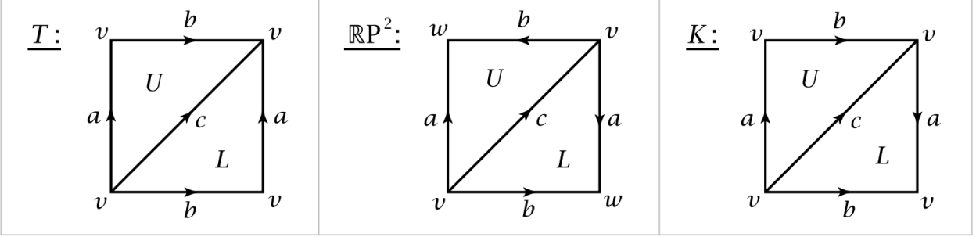
\includegraphics[width=\textwidth]{figures/chap1_1_1}
\caption[Cạnh đối diện vecto]{Cạnh đối diện vecto
\label{fig:chap1_1_1}}
\end{figure}

\indent Cắt một hình vuông theo một đường chéo sẽ tạo ra hai hình tam giác, vì vậy mỗi bề mặt này cũng có thể được dựng từ hai tam giác bằng cách xác định các cạnh của chúng theo từng cặp. Tương với một đa giác ,với bất kỳ số cạnh nào cũng có thể được cắt dọc đường chéo thành  hình tam giác. Như vậy, với đơn hình chuẩn \(n\) chiều  ∆n , dễ dàng thấy  ∆0 là một điểm, ∆1 là một đoạn thẳng, ∆2 là một tam giác, ∆3 là một tứ diện,...

\begin{figure}  
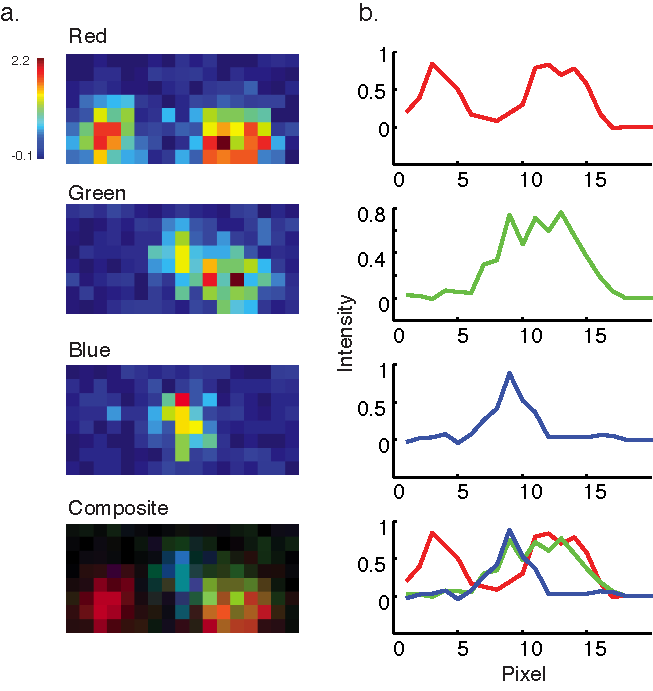
\includegraphics[width=\textwidth]{figures/fullpage}
\caption[Short figure name.]{This is a full page figure using the FPfigure command. It takes up the whole page and the caption appears on the preceding page. Its useful for large figures. Harvard's rules about full page figures are tricky, but you don't have to worry about it because we took care of it for you. For example, the full figure is supposed to have a title in the same style as the caption but without the actual caption. The caption is supposed to appear alone on the preceding page with no other text. You do't have to worry about any of that. We have modified the fltpage package to make it work. This is a lengthy caption and it clearly would not fit on the same page as the figure. Note that you should only use the FPfigure command in instances where the figure really is too large. If the figure is small enough to fit by the caption than it does not produce the desired effect. Good luck with your thesis. I have to keep writing this to make the caption really long. LaTex is a lot of fun. You will enjoy working with it. Good luck on your post doctoral life! I am looking forward to mine. \label{fig:myFullPageFigure}}
\end{figure}
\afterpage{\clearpage}


\section{This is section two}
\blindtext
\blindmathpaper

\section{This is section three}
\blindtext
\blindmathpaper
\chapter{ĐỒNG ĐIỀU KỲ DỊ}

\indent Một \(n\)-đơn hình kỳ dị trong không gian \(X\) , theo định nghĩa chỉ là một ánh xạ liên tục  \(\sigma : \Delta_n\rightarrow$X$\). \\
\indent Cho \(C_n(X)\) là nhóm \(abel\) tự do có cơ sở  \(n\)-đơn hình kỳ dị trong \(X\) . Các phần tử của \(C_n(X)\), được gọi là \(n\)-dây chuyền hoặc hơn thế nữa là \(n\)-dây chuyền kỳ dị , là tổng hữu hạn \(\sum_{i}n_i$$e_i^n$$\) với \(n_i \in \mathds{Z}\) và \(\sigma_i : \Delta_n\rightarrow$X$\) . Một ánh xạ bờ  \(\partial_n : C_n(X)\rightarrow C_{n-1} (X)\) được xác định theo cùng một công thức như trước:
\[\partial_n(\sigma) = \sum_{i}(-1)^i\sigma|[v_0, \cdots,\hat{v}_i,\cdots,v_n]\] \\
\indent Với công thức này \(\sigma|[v_0, \cdots,\hat{v}_i,\cdots,v_n]\) được coi là một ánh xạ \(\Delta_{n}-1\rightarrow$X$\) , nghĩa là, một (\(n\) − 1) - đơn hình. \\
\indent Thông thường chúng ta viết ánh xạ bờ ∂n từ \(C_n(X)\) đến \(C_{n−1} (X)\) đơn giản là \(\partial\) khi
điều này không dẫn đến sự mơ hồ nghiêm trọng. Chứng minh bổ đề \textbf{1.2.2} cũng có thể áp dụng tốt cho đơn hình kỳ dị , khi ta chỉ ra rằng \(\partial_{n}\partial_{n+1}\) = 0 hoặc chính xác hơn \(\partial^2\) = 0, vì vậy chúng ta có thể xác định nhóm đồng điều kỳ dị  \(H_n =\) Ker \(\partial_n / \) Im \(\partial_{n+1}\) . \\
\indent Rõ ràng từ định nghĩa thấy rằng các không gian đồng cấu có các nhóm đẳng cấu đơn hình kỳ dị \(H_n\) , trái ngược với trường hợp của \(H_n^{\Delta}\) . Mặt khác, vì các nhóm \(Cn(X\)) quá lớn nên số \(n\)-đơn hình  trong \(X\) thường là không thể đếm được, nó không rõ ràng rằng với một \(\Delta\) - phức \(X\) có hữu hạn các đơn hình , \(H_n(X)\) phải được sinh ra hữu hạn cho mọi \(n\), hay \(H_n(X)\) phải bằng không cho \(n\) lớn hơn số chiều của \(X\) - hai tính chất tầm thường đối với \(H_n^{\Delta} (X)\). \\
\indent Mặc dù đồng điều kỳ dị có vẻ tổng quát hơn nhiều so với đơn hình đồng điều,nhưng  nó thực sự có thể được coi là một trường hợp đặc biệt của đơn hình đồng điều bằng phương pháp sau:

\section{Định nghĩa}
\indent Với \(X\) là không gian tùy ý, ta định nghĩa phức hợp kỳ dị \(S(X)\) là \(\Delta\)-phức với một \(n\)-đơn hình \(\Delta_{\sigma}^n\) cho mỗi \(n\)- đơn hình kỳ dị \(\sigma : \Delta_n\rightarrow$X$\) với \(\Delta_{\sigma}^n\) được gắn với  (\(n\) − 1)- đơn hình  của \(S(X)\) là những hạn chế  của \(\sigma\) đối với (\(n\) − 1) -đơn hình  khác nhau trong \(\partial\Delta^n\). \\
\indent Rõ ràng từ các định nghĩa thấy  rằng \(H_n^{\Delta} S(X)\) đồng biến với \(H_n(X)\) với  \(n\), và theo nghĩa này, nhóm đồng điều kỳ dị  \(H_n(X)\) là trường hợp đặc biệt của nhóm đơn hình đồng điều. Người ta có thể coi \(S(X)\) là một mô hình \(\Delta\) - phức cho \(X\) , mặc dù nó thường là một đối tượng cực lớn so với \(X\) . \\
\indent Các chu trình trong đồng điều kỳ dị được định nghĩa theo đại số, nhưng chúng có thể được  giải thích theo hình học khi nói về ánh xạ từ các \(\Delta\)-phức hữu hạn. Để thấy rõ vấn đề này, điều quan trọng đầu tiên là \(n\) - dây chuyền kỳ dị  luôn có thể viết dưới dạng \(\sum_{i}\varepsilon_i\sigma_i\) với với \(\varepsilon_i\) = \(\pm\)1 cho phép lặp lại \(n\)-đơn hình kỳ dị \(\sigma_i\) . Cho \(n\)-dây chuyền \(\xi\) = \(\sum_{i}\varepsilon_i\sigma_i\) khi chúng ta tính \(\partial\xi\)  là tổng của (\(n\)-1)-đơn hình kỳ dị với dấu \(\pm\)1. Có thể tồn tại một số cặp triệt tiêu bao gồm hai  (\(n\) − 1) - đơn hình kỳ dị giống hệt nhau trái dấu. Chọn một tập hợp tối đa các cặp triệt tiêu như vậy, xây dựng một  ∆- phức  n chiều \(K_{\xi}\) từ một tổ hợp  rời rạc của \(n\) - đơn hình \(\Delta_i^n\) ,cho mỗi \(\sigma_i\) , bằng cách xác định các cặp (\(n\)−1) chiều tương ứng với các cặp triệt tiêu đã chọn. \(\sigma_i\)  của sau đó tạo ra một ánh xạ \(K_{\xi} \rightarrow X\) . Nếu như \(\xi\) là một chu trình, tất cả (\(n\)−1)  chiều của \(\Delta_i^n\)  được xác định theo cặp. Như vậy \(K_{\xi}\) là một đa tạp, đồng cấu với $\mathsf{R}$ , gần với tất cả các điểm trong phần bù của (n − 2) - khung \(K^{n-2}_{\xi}\) của \(K_\xi\) . \\
\indent Đặc biệt, các yếu tố của \(H1(X)\) được biểu diễn bằng tập hợp các vòng định hướng trong \(X\) , và các phần tử của \(H_2(X)\) được biểu diễn bằng ánh xạ của các bề mặt định hướng khép kín vào \(X\) .Có thể chỉ ra rằng 1 chu kỳ được định hướng \(\amalg_{\alpha}S^1_{\alpha} \rightarrow X\) là không trong \(H(X)\) nếu nó mở rộng thành ánh xạ của một bề mặt định hướng nhỏ gọn với biên \(\amalg_{\alpha}S^1_{\alpha} \rightarrow X\) vào \(X\).

\section{Mệnh đề}
\indent Tương ứng với sự phân tách của một không gian \(X\) thành các thành phần cung của nó \(X_{\alpha}\), có một đẳng cấu của \(H_n(X)\) với tổng trực tiếp \(\bigoplus_{\alpha}H_n(X_{\alpha})\). \\
\textbf{Chứng minh:} \\
\indent Vì một đơn hình đồng điều luôn có ảnh liên thông cung , \(C_n(X)\) chia thành tổng trực tiếp của các nhóm con của nó \(C_n(X_{\alpha})\). Các ánh xạ biên \(\partial_n\) bảo toàn tổng trực tiếp này phân tách, lấy \(C_n(X_{\alpha})\) thành \(C_{n−1} (X_{\alpha})\), do đó Ker \(\partial_n / \) và \(Im\) \(\partial_{n+1}\) chia tương tự như tổng trực tiếp, do đó các nhóm đồng điều cũng tách ra, \(H_n(X) \approx \bigoplus_{\alpha}H_n(X_{\alpha})\).


\section{Mệnh đề}
\indent Nếu \(X\) khác rỗng và liên thông cung thì \(H_0(X) \approx \mathds{Z} \) . Do đó đối với không gian \(X\) bất kỳ , \(H_0 (X)\) là tổng trực tiếp của  \(\mathds{Z}\) , cho mỗi thành phần cung của \(X\). \\
\textbf{Chứng minh: } \\
\indent Theo định nghĩa, \(H_0(X) = C_0(X)/Im\partial_0\)  khi  \(\partial_0\) = 0. Xác định một phép đồng cấu \\ \(\varepsilon : C_0(X) \rightarrow \mathds{Z} \) được cho bởi \(\varepsilon(\sum_{i}n_{i}\sigma_i) = \sum_{i}n_i\) .Ta nói , \(Ker\) \(\varepsilon = Im \partial_1\) nếu \(X\) liên thông cung  và do đó \(\varepsilon\) tạo ra một đẳng cấu \(H_0 (X) \approx \mathds{Z}\) . \\
\indent Ta sẽ chứng minh điều đó như sau: \\
Đầu tiên, ta thấy Im \(\partial_1 \subset\) Ker \(\varepsilon\)  khi đối với 1-đơn hình kỳ dị \(\sigma: \Delta
_1 \rightarrow X\) ta có
\[\varepsilon \partial_1(\sigma) = \varepsilon(\sigma|[v_1] - \sigma|[v_0]) = 1-1 = 0\]
Ngược lại, Ker \(\varepsilon \subset \) Im \(\partial_1\), giả sử \(\varepsilon(\sum_{i}n_{i}\sigma_i)=0\) , khi đó \(\sum_{i}n_i=0\). \(\sigma_i\) của 0-đơn hình đồng điều là điểm của \(X\). Chọn \(\uptau_i: I \rightarrow X\) từ \(x_0\) đến \(\sigma_i(v_0)\) đặt \(\sigma_0\) là 0-đơn hình kỳ dị với ảnh \(x_0\). Chúng ta có thể xem nó dưới dạng 1-đơn hình kỳ dị, ánh xạ \(\uptau_i : [v_0 , v_1]\rightarrow X\) , và khi đó chúng ta có \(\partial \uptau_i = \sigma_i\) - \(\sigma_0\) . \\
Do đó, \(\partial(\sum_{i}n_{i}\uptau_i) = \sum_{i}n_{i}\sigma_i\) - \(\sum_{i}n_{i}\sigma_0\) =  \(\sum_{i}n_{i}\sigma_i\)  khi \(\sum_{i}n_{i}\) = 0. Như vậy, \(\sum_{i}n_{i}\sigma_i\) là một biên, chứng tỏ rằng \(Ker\) \(\varepsilon \subset \) \(Im\) \(\partial_1\) . \\

\section{Mệnh đề}
\indent Nếu \(X\) là một điểm thì \(H_n(X) = 0\) với \(n > 0\) và \(H_0(X) \approx \mathds{Z} \)  . \\
\textbf{Chứng minh:} \\
Trong trường hợp này, có một \(n\) đơn hình duy nhất \(\sigma_n\) cho mỗi \(n\) và \(\partial(\sigma_n)=\) \(\sum_i(-1)^{i}\sigma_{n-1}\) , tổng của \(n\) + 1 số hạng, do đó bằng 0 với \(n\) lẻ và \(\sigma_{n-1}\) với \(n\) chẵn, \(n\) ≠ 0. Do đó ta có dãy phức:
\[\cdots \longrightarrow \mathds{Z}  \xlongrightarrow[]{\approx} \mathds{Z} \xlongrightarrow[]{0} \mathds{Z} \xlongrightarrow[]{\approx} \mathds{Z} \xlongrightarrow[]{0} \mathds{Z} \longrightarrow 0\]
với các ánh xạ biên  xen kẽ các đẳng cấu và ánh xạ tầm thường, ngoại trừ ở  \(\mathds{Z}\)  cuối cùng. Các nhóm đồng điều của phức hợp này là tầm thường ngoại trừ \(H_0 \approx \mathds{Z}  \) .


\begin{savequote}[75mm] 
Nulla facilisi. In vel sem. Morbi id urna in diam dignissim feugiat. Proin molestie tortor eu velit. Aliquam erat volutpat. Nullam ultrices, diam tempus vulputate egestas, eros pede varius leo.
\qauthor{Quoteauthor Lastname} 
\end{savequote}

\chapter{Consectetuer adipiscing elit}

\newthought{Lorem ipsum dolor sit amet}, consectetuer adipiscing elit. Morbi commodo, ipsum sed pharetra gravida, orci magna rhoncus neque, id pulvinar odio lorem non turpis. Nullam sit amet enim. Suspendisse id velit vitae ligula volutpat condimentum. Aliquam erat volutpat. Sed quis velit. Nulla facilisi. Nulla libero. Vivamus pharetra posuere sapien. Nam consectetuer. Sed aliquam, nunc eget euismod ullamcorper, lectus nunc ullamcorper orci, fermentum bibendum enim nibh eget ipsum. Donec porttitor ligula eu dolor. Maecenas vitae nulla consequat libero cursus venenatis. Nam magna enim, accumsan eu, blandit sed, blandit a, eros.

\blindtext

\section{This is section one}
\blindtext
\blindmathpaper

\section{This is section two}
\blindtext
\blindmathpaper

\singlespacing

\clearpage
\bibliography{refs}
\addcontentsline{toc}{chapter}{Tài liệu tham khảo}
\bibliographystyle{plainnat}

\begin{appendices}
\chapter{This is title of appendix A}
\blindmathpaper
\chapter{This is title of appendix B}
\blindmathpaper
\end{appendices}

\end{document}
